% !TEX root = ../Masterarbeit.tex
\chapter{Grundlagen \& Begriffsbestimmung}
In diesem Kaptiel werden die Grundlagen beschrieben, auf die der Hauptteil aufbaut. Zudem behandelt das Kapitel die Begriffsbestimmung und die genauen Eigenschaften reaktiver Systeme.\\
Da die Umsetzung reaktiver Systeme gewisse Programmierparadigmen vorausgesetzt, werden diese nach den reaktiven Merkmalen erklärt.

\section{Eigenschaften reaktiver Systeme}
Reaktive Anwendungen haben die Eigenschaften folgendes zu leisten bzw. folgende Punkte zu erfüllen~\cite[S.~19ff]{kuhn_reactive_2015}~\cite[S.~6]{vernon_reactive_2016}.\\

\textbf{Eine reaktive Anwendung muss\ldots}
\begin{enumerate}
\item \ldots \textbf{auf variable Belastung reagieren (siehe~\fullref{subsec:elastic}).} Das System ist automatisch in der Lage dynamische Skalierung durchzuführen und nicht benötigte Ressourcen wieder freizugeben.
\item \ldots \textbf{auf Fehler reagieren (siehe~\fullref{subsec:resilient}).} Die Software ist von Grund auf widerständsfähig gegenüber Fehlerzuständen. Die Wiederherstellung des Normalzustand erfolgt automatisch.
\item \ldots \textbf{auf Nutzer oder Komponenten reagieren (siehe~\fullref{subsec:responsive}).} Jede Anfrage wird in der geforderten Antwortzeit oder schneller bearbeitet.
\item \ldots \textbf{auf Nachrichten reagieren (siehe~\fullref{subsec:messagedriven}).} Das System verwendet asynchrone Nachrichtenübermittlung zwischen den Komponenten und ist somit \textit{message-driven}.
\end{enumerate}

Die nachfolgenden Abschnitte erklären die Merkmale im Detail und zeigen den Zusammenhang zwischen ihnen.

\subsection{Elastic}\label{subsec:elastic}
Eine reaktive Anwendung muss auf variable Belastung ebenso variable bzw. dynamisch reagieren können. Wird Beispielsweise ein Online Shop in einer Fernsehwerbung oder von einem bekannten Blog erwährt, müssen kurzfristig sehr viele Anfragen angemessen und zufriedenstellend verarbeitet werden~\cite[S.~39]{kuhn_reactive_2015}.\\
Um die gewünschten und geforderten Antwortzeiten einzuhalten, muss das System skalieren. Traditionellerweise ist hiermit \textit{scaling up} gemeint. Aufgrund der heutigen Anforderungen stößt man schnell an die Grenzen eines einzelnen Hosts. Dementsprechend muss das System nicht nur vertikal, sondern auch horizontal skalieren. Dazu muss die Anwendung auf mehrere Nodes verteilt werden~\cite[S.~7]{vernon_reactive_2016}. Es ist deshalb wichtig, die Teilaufgaben einer Applikation zu identifizieren und auf einzelne Komponenten aufzuteilen, die dann wie bereits erwähnt auf einzelne Nodes verteilt werden können~\cite[S.~40]{kuhn_reactive_2015}.\\
Das Reactive Manifesto fordert zudem auch, das System so zu gestalten, dass es \textit{scaling down} fähig ist. Das bedeutet ungenutze und nicht benötigte Ressourcen müssen wieder freigegeben werden. Dadurch kann man ein hochskalierbares und reaktives System kosteneffizient betreiben. Im Reactive Manifesto hat man sich auf den Begriff \textit{elastic} geeinigt, um deutlich zu machen, dass man in beide Richtungen skalieren kann. Bei reaktiven Applikationen spricht man deshalb von elastischer bzw. dymanischer Skalierung~\cite[S.~8]{vernon_reactive_2016}. Für die Software bedeutet dies, dass einzelne Nodes jederzeit hinzugefügt und entfernt werden können. Als Folge dessen muss das System \textit{location transparent} sein. Insofern dürfen dessen Komponenten und Funktionen nicht abhängig von einem Host sein~\cite[S.~8]{vernon_reactive_2016}. 

% TODO Little's Law
% TODO Infrastructure as a Service oder Cloud Computing; Enterprise IT OpenStack

\pagebreak

\subsection{Resilient}\label{subsec:resilient}
Eine Software \textit{resilient} (dt. widerstandsfähig) zu entwickeln bedeutet nicht, dass die Software fehlerfrei ist. Es bedeutet, dass die Software sich von einem Fehlerzustand erholen kann~\cite[S.~6]{vernon_reactive_2016}.\\
Schon bei dem Entwurf von Software wird versucht Fehler von vornherein zu bedenken und mit ihnen sinnvoll umzugehen. Folgendes Zitat von Jonas Bonér macht deutlich, wie wichtig die Widerstandsfähigkeit einer Software ist.

\begin{quotation}
Without resilience, nothing else matters. If your beautiful, production-grade, elastic, scalable, highly concurrent, non-blocking, asynchronous, highly responsive and performant application isn't running, then you're back to square one. It starts and ends with resilience.~\citetext{Bonér, Jonas; 2015}
\end{quotation}

Im Grunde ist diese Aussage trivial. Eine Software, die nicht läuft ist unbrauchbar --- egal wie komplex und durchdacht die Architektur auch sein mag.\\
Es ist aber nicht nur die eigene Software, die betroffen sein kann. Andere externe Softwarekomponenten, von denen man abhängt oder auch die Hardware kann im laufenden Betrieb Probleme bereiten~\cite[S.~33]{kuhn_reactive_2015}.\\
Der Schluss, den man daraus ziehen sollte, lautet deshalb nicht, ob ein Fehler auftritt sondern viel mehr wann und wie häufig das passiert. Für den Benutzer ist es nebensächlich, warum ein interner Fehler aufgetreten ist. Die Anwendung wird in diesem Moment nicht das tun, was der Benutzer von ihr erwartet~\cite[S.~33]{kuhn_reactive_2015}.\\

Im Reactive Manifesto hat man für dieses Problem bzw. die Eigenschaft ganz bewusst den Begriff \textit{resilience} und nicht \textit{reliability} (dt. Ausfallsicherheit) gewählt. Man möchte deutlich machen, dass es nahezu unmöglich ist, ein ausfallsicheres System zu schaffen. Deshalb setzt man auf widerstandsfähige Systeme, welche mit Fehlerzuständen sinnvoll umgehen und vorallem sich von dieses wieder erholen. Folglich ist ein reaktives System nicht nur \textit{fault tolerant} (dt. Fehler tolerant), sondern geht noch einen Schritt weiter~\cite[S.~34]{kuhn_reactive_2015}.\\

Um die Eigenschaft \textit{resilience} zu erfüllen, muss das System in Komponenten aufgeteilt und anschließend verteilen (engl.~\textit{distribute}) werden. Zusätzlich ist es notwendig, die verteilen Komponenten von einander abzuschotten (engl.~\textit{compartmentalize})~\cite[S.~34]{kuhn_reactive_2015}~\cite[S.~7]{vernon_reactive_2016}.\\
Aufgrund der verteilten und abgeschottenten Komponenten können Fehler isoliert werden. Hierfür führt man das Prinzip der \textit{supervision} ein. Nach- bzw. untergeordnete Komponenten informieren ihren \textit{supervisor} im Falle eines Fehlers. Dieser hat nun die Möglichkeit die Subkomponente z.B. neuzustarten oder eine erneute Anfrage zustellen. 

\subsection{Responsive}\label{subsec:responsive}
Eine reaktive Anwendung muss zu jederzeit auf jede Anfragen reagieren. Das heißt, die Anwendung ist jederzeit \textit{responsive} (dt. antwortbereit). Anfragen können nicht nur durch einen Benutzer ausgelöst werden, sondern können auch von anderen Diensten oder Komponenten initiert werden. Als Client einer reaktiven Anwendung muss man sich drauf verlassen können, dass eine Antwort in einem festgelegten Zeitraum eintrifft. Das bedeutet es müssen \textit{timeouts} festgelegt werden, nachdem eine Anfrage für fehlerhaft erklärt wird.\\
Ist eine Anwendung nicht \textit{elastic} (siehe~\ref{subsec:elastic}) und/oder nicht \textit{resilient} (siehe~\ref{subsec:resilient}) kann sie auch nicht \textit{responsive} sein. Eine reaktive Anwendung muss unter Last skalieren, um die geforderte maximale Antwortzeit einzuhalten oder ein Systemausfall zu vermeiden. Gleichzeitig eingehende Anfragen müssen parallel verarbeitet werden können und dürfen nicht von langsamen Anfragen blockiert werden. Fallen Komponenten aus, z.B. durch einen unvorhergesehenen Hardwarefehler, könnten diese aufgrund der \textit{location transparency} auf einem anderen Node neu gestartet werden, um die \textit{responsivenes} aufrechtzuerhalten.

\pagebreak

\subsection{Message-driven}\label{subsec:messagedriven}
Um die bereits erwähnten Eigenschaften \textit{elasticity} (\ref{subsec:elastic}), \textit{resilience} (\ref{subsec:resilient}), sowie die daraus folgende \textit{responsiveness} (\ref{subsec:responsive}) zu erfüllen, müssen reaktive Anwendungen \textit{message-driven} sein~\cite{webber_what_2014}~\cite[S.~43]{kuhn_reactive_2015}. Somit ist die Basis einer reaktiven Anwendung die vierte Eigenschaft aus dem Reactive Manifesto~\cite{boner_reactive_2014}.\\
Ist ein System \textit{message-driven} erfolgt die Kommunikation ausschließlich über asynchronen Nachrichtenaustausch zwischen den Komponenten, wodurch eine strikte Abgrenzung der Komponenten erfolgt. Durch die Abstraktion der Kommunikation wird eine lose Kopplung zwischen den Komponenten sichergestellt. Darüber hinaus sind die Komponenten voneinander isoliert, wodurch es möglich ist, Fehler als Nachrichten zu delegieren (siehe~\ref{subsec:resilient}).\\
Durch den expliziten Nachrichtenaustausch kann über \textit{message queues} und \textit{flow control} die Last verteilt und kontrolliert werden. Ebenso wird die gewünschte \textit{location transparency} durch die Entkopplung über den asynchronen Nachrichtenaustausch ermöglicht~\cite{boner_reactive_2015}~\cite[S.~43]{kuhn_reactive_2015}.\\
Die folgende Abbildung (Abb. \ref{fig:four-traits}) soll den Zusammenhang der vier Merkmale nochmals verdeutlichen. Neben dem wohl wichtigsten Ziel der \textit{responsiveness} hat die reaktive Architektur den Vorteil, wartbare und auch erweiterbare Anwendungen zu schaffen. Jedoch werde die weiteren Ziele nur in der Einleitung des Reactive Manifestos und nicht als Kerneigenschaft formuliert~\cite{boner_reactive_2014}. Die Ziele erreicht man durch die Eigenschaften \textit{elasticity} und \textit{resilience}. Die Grundvoraussetzung ist im wesentlichen die asynchrone, nicht-blockierende und nachrichtengetriebene Kommunikation (\textit{message-driven}).

\begin{figure}[H]
 \centering
 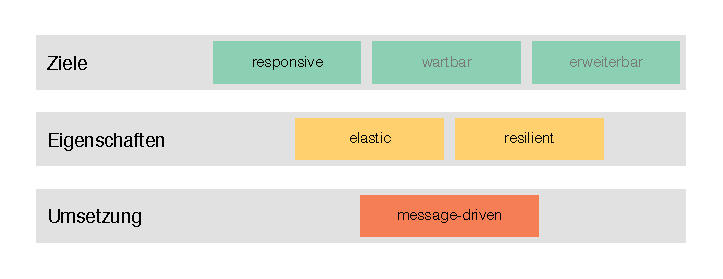
\includegraphics[width=1.0\textwidth]{3-Grundlagen/four-traits/four-traits.eps}
 \caption{Die vier Merkmale einer reaktiven Anwendung \cite{kuhn_code_2015}}
 \label{fig:four-traits}
\end{figure}

\pagebreak

\section{Parallelität \& Nebenläufigkeit}

\subsection{Notwendigkeit}\label{subsec:notwendigkeit}
Die Prozessorhersteller sind in den letzten Jahren an gewisse Grenzen bei der Entwicklung von CPUs gestoßen. Seit 2003 stagniert die Entwicklung hinsichtlich der Taktraten von Prozessoren. Die Beobachtung von Gordon Moore (\enquote{Moore's Law}) scheinen nach wie vor seine Gültigkeit zu haben und die Zahl der Transistoren verdoppelt sich ungefähr alle zwei Jahre. Diese werden jedoch nicht genutzt, um eine einzelne CPU schneller zu machen. Hersteller setzen stattdessen seit einigen Jahren auf Multicore-Architekturen~\cite[S.~1]{butcher_seven_2014}~\cite[S.~108]{vernon_reactive_2016}~\cite{sutter_free_2004}.\\
Herb Sutter veröffentlichte diesbezüglich 2004 einen Artikel mit dem Titel \enquote{The free lunch is over}. Mit \enquote{free lunch} bezog er sich auf die Tatsache, dass sequenzielle Anwendungen ohne das Zutun von Entwicklern aufgrund der damals noch steigenden Taktraten schneller wurden --- vielmehr schneller ausgeführt wurden.\\
Im Hinblick auf die Multicore-Prozessoren und der mehr oder weniger stagnierenden Taktraten müssen Anwendungen ihre Aufgaben und Teilaufgaben nebenläufig und parallel ausführen, um die heutigen und zukünftigen Prozessoren optimal auszulasten~\cite[S.~45]{kuhn_reactive_2015}~\cite{sutter_free_2004}~\cite[S.~1]{butcher_seven_2014}.\\
Sequenzielle Programme werden Schritt für Schritt ausgeführt. Genauer gesagt, erfolgt die Ausführung der einzelnen Befehle nach einer vorgegebenen Reihenfolge. Folglich profitiert ein sequenzielles Programm nicht von modernen Multicore-Prozessoren. Hier kommen nun Nebenläufigkeit (engl. concurrency) und Parallelität (engl. parallelism) ins Spiel~\cite[S.~3]{butcher_seven_2014}.\\

Die Welt, in der wir leben, ist hochgradig parallel. Während wir Menschen mit dem Auto über eine Autobahn fahren, nehmen wir, wenn auch meist nur unterbewusst, viele unterschiedliche Dinge gleichzeitig wahr. Während wir uns sportlich betätigen, hören wir meistens gleichzeitig zum Laufen Musik, um uns anzuspornen. Während wir zum Zeitvertreib auf unserem Smartphone ein Spiel spielen, kann es derweil trotzdem Emails abrufen. Würden diese Prozesse sequentiell und nicht parallel abläufen, hätten wir vermutlich schon längst hunderte Autounfälle in unserem Leben verursacht.\\
Blickt man nun auf Parallelität im Bezug auf Prozessoren und Software, wird zwischen mehreren Ebenen von Parallelität unterscheiden. Zum Beispiel kann ein Singlecore-Prozessor aufgrund von Technologien, wie Pipelining mehrere Schritte parallelisieren. Ebenso sind Multitasking Betriebssysteme in der Lage auf einem Singlecore-Prozessor mehrere Prozesse nebenläufig bzw. quasi-parallel auszuführen~\cite[S.~3~\&~S.~4]{butcher_seven_2014}. Der folgende Abschnitt bezieht sich auf Parallelität im Bezug auf Multicore-Prozessoren und wie diese erreicht werden kann.\\
Nebenläufigkeit und Parallelität werden fälschlicherweise oft als Synonyme verwendet. Die beiden Begriffe sind verwandt, beschreiben jedoch verschiedene Sachverhalte.\\
Aus der Sicht eines Problems (Problemdomäne), bedeutet Nebenläufigkeit das Bearbeiten gleichzeitig oder annähernd gleichzeitig eintreffender Ereignisse. Im Gegensatz dazu bezieht sich Parallelität auf die beschleunigte Lösung eines Problems durch Fragmentierung und der simultanen Bearbeitung der Teilprobleme~\cite[S.~1~\&~S.~2]{butcher_seven_2014}~\cite[S.~15]{vernon_reactive_2016}.\\
Rob Pike formulierte den Unterschied zwischen Nebenläufigkeit und Parallelität wie folgt:

\begin{quotation}
  Concurrency is about dealing with lots of things at once. Parallelism is about doing lots of things at once. [...] Concurrency provides a way to structure a solution to solve a problem that may (but not necessarily) be parallelizable~.
\cite[S.~10]{pike_concurrency_2012}
\end{quotation}

Im Grunde bedeutet das, die Nebenläufigkeit beschreibt die Koordination mehrerer unabhängiger Abläufstränge (\textit{threads of control}). Parallelität hingegen die simultane bzw. gleichzeitige Ausführung von Berechnungen, die nicht zwingendermaßen zusammenhängen~\cite[S.~8-9]{pike_concurrency_2012}~\cite[S.~3]{butcher_seven_2014}.\\
Kann ein Problem bzw. eine Anwendung nebenläufig beschrieben bzw. entworfen werden, ist es möglich, die Anwendung parallel und entsprechend effizienter auszuführen~\cite[S.~19~\&~S.~30]{pike_concurrency_2012}.\\
Die effizientere Ausführung hat jedoch Grenzen und diese hängen von den sequenziellen Segmenten ab. Gene Amdahl stellte hierfür bereits 1967 ein Modell auf (\enquote{Amdahl's Law}), welches den Grad der Beschleunigung einer Anwendungen durch dessen parallele Anteile beschreibt. So zum Beispiel kann eine Anwendung, die nur zu 90~\% parallelisiert ist, maximal um den Faktor 10 schneller ausgeführt werden~\cite{amdahl_validity_1967}. Dies zeigt, wie wichtig es ist, auf sequenzielle Abschnitte zu achten und diese möglichst zu vermeiden.\\

Die Art und Weise, wie wir heute mit der digitalen Welt interagieren, ist nebenläufig und parallel. Demnach müssen Anwendungen ebenso nebenläufig sein, um den Anforderungen zu entsprechen~\cite[S.~5]{butcher_seven_2014}~\cite[S.~3~\&~S.~178]{armstrong_programming_2013}.\\
Ein nebenläufiges Design erlaubt es einer Anwendung \textit{responsive}, fehlertolerant und effizient zu sein~\cite[S.~4~\&~S.~6]{butcher_seven_2014}~\cite[S.~6]{armstrong_programming_2013}.\\
Nur eine Anwendung, die nebenläufig mehrere Ereignisse verarbeiten kann, ist in der Lage \textit{responsive} zu sein. Beispielsweise kann ein Browser mehrere Webseiten gleichzeitig (nebenläufig) laden und der Benutzer hat die Möglichkeit währenddessen eine weitere Seite zu öffnen, ohne auf die Beendigung der anderen Ladevorgänge warten zu müssen. Verteilt man eine Anwendung auf mehrere Nodes, muss diese implizit nebenläufig sein --- oder anders ausgedrückt, nebenläufiges Design erlaubt das Verteilen auf mehrere Nodes. Die Möglichkeit eine Anwendung zu verteilen und somit redundant zu betreiben, ist Basis für \textit{resilience} und \textit{elasticity}~\cite[S.~6]{butcher_seven_2014}~\cite[S.~6~\&~S.~7]{armstrong_programming_2013}.\\

Zusammenfassend kann man diesem Abschnitt entnehmen, dass reaktive Anwendungen per Definition nebenläufig entworfen und umgesetzt werden müssen, um die Eigenschaften des Reactive Manifestos zu erfüllen.

\pagebreak

\subsection{Share nothing}\label{subsec:sharenothing}
Nebenläufige Komponenten teilen sich traditionellerweise Daten, um zu interagieren. Der Zugriff auf den sogenannten \textit{shared memory} kann nebenläufig und parallel erfolgen, deshalb müssen die Operationen synchroniziert werden. Hierfür nutzt man das Konzept der \textit{mutual exclusion}. Man stellt über sogenannte \textit{locks} sicher, dass nur ein \textit{thread of control} zur selben Zeit auf die Daten zugreifen kann~\cite[S.~10]{butcher_seven_2014}. Der Zugriff auf die Daten erfolgt somit sequenziell, weshalb die Vorteile einer nebenläufigen Anwendung an dieser Stelle zunichtegemacht werden (siehe \fullref{subsec:notwendigkeit})~\cite[S.~45]{kuhn_reactive_2015}. Zudem haben Anwendungen mit \textit{shared memory} unteranderem mit Problemen wie \textit{memory corruption}, \textit{deadlocks} und \textit{starvation} zu kämpfen~\cite[S.~117]{vernon_reactive_2016}.\\
In reaktiven Anwendungen müssen Komponenten voneinander isoliert sein (siehe \fullref{subsec:resilient}), folglich dürfen sie keine Informationen teilen (\textit{share nothing}). Um mit einer anderen Komponente zu interagieren, müssen reaktiven Komponenten asynchrone Nachrichten ausgetauschen (siehe \fullref{subsec:messagedriven}). Dieses Konzept der nebenläufigen Interaktion wird \textit{message passing} genannt und ist eine Alternative zum \textit{shared memory}. Der Vorteil ist, da Informationen nur durch den expliziten Nachrichtenaustausch geteilt werden, benötigt man keine \textit{mutual exclusion} und hat somit eine \textit{lock-free concurrency}.\\
Durch diese lose Kopplung erhält man klare Grenzen zwischen den Komponenten. Dies führt zu Kapselung von Fehlern, Implementierungsdetails und Verantwortlichkeiten. Desweiteren hilft es bei der Umsetzung von \textit{location transparency} und effizienteren Nutzung der Ressourcen~\cite[S.~45]{kuhn_reactive_2015}.

\pagebreak

\subsection{Kommunikation \& Interaktion}
Eine reaktive Anwendung ist \textit{message-driven}. Hierzu müssen Nachrichten zwischen den Komponenten ausgetauscht werden. Es gibt zwei Möglichkeiten der Kommunikation. Zum einen die synchrone und zum anderen die asynchrone Kommunikation.

\subsubsection{Synchrone Kommunikation}
Die traditionelle Kommunikation zwischen zwei Komponenten ist die synchrone Kommunikation. Komponente \textit{a} ruft eine Funktion \textit{f} der Komponente \textit{b} auf. Die Berechnung erfolgt synchron und deshalb wartet Komponente \textit{a} auf das Ergebnis und kann dann erst die weiteren Schritte sequenziell abarbeiten. Die weiteren Schritte müssen jedoch nicht von dem Ergebnis der Funktion \textit{f} abhängig sein und trotzdem wird deren Berechnung blockiert. Sollte bei dem Funktionsaufruf ein Fehler auftreten, werden die nachfolgenden Befehle nicht ausgeführt. Die Komponente \textit{b} ist von diesem Fehler ebenfalls betroffen, solange die beiden Komponenten im gleichen Thread ausgeführt werden. Folglich sind die Komponenten \textit{a} und \textit{b} stark voneinander abhängig~\cite[S.~22]{kuhn_reactive_2015}.\\
Es wird klar, dass diese Art der Kommunikation für \textit{responsivness}, \textit{resilience} und \textit{elasticity} nicht förderlich ist~\cite[S.~46]{kuhn_reactive_2015}.

\subsubsection{Asynchrone Kommunikation}
Sobald die Komponenten \textit{a} und \textit{b} verteilt werden, löst sich die angesprochene Kopplung. Dies kann durch Ausführung in jeweils eigenen Threads geschehen oder durch die Verteilung auf mehrere Nodes. Dies ist ein notwendiger Schritt hinzu einer reaktiven Anwendung~\cite[S.~22]{kuhn_reactive_2015}.\\
Innerhalb verteilter Anwendungen ist synchrone Kommunikation (in seiner einfachsten Form ein Funktionsaufruf), wie bereits erwähnt, nicht wünschenswert. Oft werden die Gegebenheiten lokaler Funktionsaufrufe auf eine verteile Netzwerkkommunikation übertragen. Peter Deutsch formulierte diesbezüglich sieben Irrtümer bzw. Annahmen, die im Bezug auf verteile Systeme gemacht werden. Zum Beispiel die Annahme ein Netzwerk wäre ausfallsicher oder die Latenz der Netzwerkkommunikation geht gegen null. Diese Annahmen treffen selbstverständlich nicht zu~\cite[S.~1]{rotem_fallacies_2008}. In einem weiteren Artikel beschäftigen sich Waldo et al ebenfalls mit der Kommunikation in einem verteilten System und kommen zu dem Schluss, dass vorallem unvorhersehbare Latenz und teilweiser Ausfall der Kommunikation (engl. \textit{partial failure}) unvermeidbar sind~\cite{waldo_note_1994}.\\
Im Gegensatz zur synchronen Kommunikation führt der Sender bei einer asynchronen Kommunikation seine Aktivitäten und Berechnungen fort und wartet nicht auf die Empfangsbestätigung oder Antwort des Empfängers. Der Empfänger selbst verarbeitet die Nachrichten meist auch asynchron. Eingehende Nachrichten werden zuerst in einer \textit{message queue} bis zur Bearbeitung zwischengelagert. Man spricht auch von asynchronener und nicht blockierender Kommunikation. Durch die asynchrone Programmierung werden die Ressourcen nicht durch unvermeidbares Warten blockiert sondern effektiver genutzt~\cite[S.~48]{kuhn_reactive_2015}.\\

Aufgrund des \textit{share nothing} Prinzips (siehe~\ref{subsec:sharenothing}) müssen Komponenten über Nachrichten miteinander interagieren. Der Abschnitt hat gezeigt, dass diese Interaktion asynchron und nicht blockierend ablaufen sollte, um die Ressourcen effizient zu nutzen~\cite[S.~48~\&~S.~49]{kuhn_reactive_2015}.

\pagebreak

\section{Funktionale Programmierung}
Funktionale Programmierung ist ein Programmierparadigma, bei diesem die Anwendungen ausschließlich aus Ausdrücken (engl. \textit{expressions}) bzw. Funktionen bestehen. Diese Funktionen haben keine Seiteneffekte, man nennt diese deshalb auch \textit{pure functions}. Funktionen werden zudem behandelt, wie übliche Datentypen (z.B. Integer oder Boolean) und können Variablen zugewiesen oder als Funktionswert übergeben werden. Man spricht deshalb von sogenannten \textit{higher order functions}~\cite[S.~50]{butcher_seven_2014}~\cite[S.~3~\&~S.~19]{chiusano_functional_2015}.\\
Folgende Abschnitte sollen gewisse Grundkonzepte der funktionalen Programmierung erklären und ihren Bezug zu reaktiven Anwendungen deutlich machen. 

\subsection{Immutable}
In traditioneller imperativer Programmierung wird meist von den so genannten veränderbaren Zuständen Gebrauch gemacht. (engl.~\textit{mutable state}). Ein veränderbarer Zustand ist eine Variable, die jederzeit modifiziert werden kann. Im Abschnitt zu \textit{share nothing} (\ref{subsec:sharenothing}) wurde bereits deutlich gemacht, dass veränderbarer \textit{shared memory} bzw. \textit{shared mutable state} bei nebenläufigen Anwendungen zu verschiedenen Problemen führen kann. Funktionale Programmierung versucht \textit{mutable state} von vornherein zu verhindern~\cite[S.~50]{butcher_seven_2014}.\\
Ist eine Variable \textit{immutable} bedeutet das, sie ist nach dem initialen Setzen eines Wertes nicht mehr veränderbar. Der gleichzeitige Zugriff auf einen \textit{shared immutable state} muss somit nicht mehr synchronisiert werden, da die Variable nur einmal beschrieben werden kann~\cite[S.~50]{butcher_seven_2014}~\cite[S.~62]{kuhn_reactive_2015}.

\pagebreak

\subsection{Pure functions}
Die sogenannten \textit{pure functions} sind Funktionen ohne Seiteneffekte. Eine \textit{pure function} liefert bei gleicher Eingabe auch immer das gleiche Ergebnis~\cite[S.~61]{kuhn_reactive_2015}. Eine Funktion, die eine global definierte Zählvariable inkrementiert, hat somit Seiteneffekte. Desweiteren darf eine \textit{pure function} keine höheren Datentypen, wie Objekte oder Listen verändern. Auch der Zugriff auf Netzwerk oder Dateisystem gilt als Seiteneffekt~\cite[S.~3]{chiusano_functional_2015}~\cite[S.~62]{kuhn_reactive_2015}.
Der Vorteil von \textit{pure functions} ist, dass der Aufruf durch das Ergebnis ersetzt werden kann. Verallgemeinert man dieses Prinzip auch auf Ausdrücke, spricht man von der sogenannten \textit{referential transparency}~\cite[S.~9]{chiusano_functional_2015}~\cite[S.~62]{kuhn_reactive_2015}. Folgendes Beispiel zeigt eine Funktion die zwei Zahlen addiert (\ref{lst:lst1}). Diese Funktion ändert keine bestehenden Variablenwerte und hat auch sonst keinerlei Seiteneffekte. Der Aufruf dieser Funktion kann folglich mit dem Ergebnis ersetzt werden, wie die letzte Zeile des Beispiels zeigt.

\begin{lstlisting}[caption={Beispiel für eine \textit{pure funcition}},label={lst:lst1}]
def add(a: Int, b: Int): Int = {
  return a + b
}

add(add(1, 2), add(3, 4))
// = (1 + 2) + (3 + 4) = 10

add(3, 7)
// = 3 + 7 = 10
\end{lstlisting}

Dieses einfache Beispiel nutzt wiederum eine \textit{pure functions}, die bereits durch die Programmiersprache, in diesem Fall Scala, bereitgestellt wird. Die Addition zweier Zahlen durch den \textit{+} Operator. Auch in nicht funktionalen Sprachen, gibt es viele Ausdrücke und \textit{pure functions}, die die \textit{referential transparency} wahren. Zum Beispiel die mathematischen Operatoren oder die Funktion zur Bestimmung der Länge einer Zeichenkette --- meist \textit{length} genannt.\\

Ein weiteres Beispiel für die \textit{referential transparency} sind Funktionen, die einen bestehenden Wert kopieren und bei diesem Vorgang Veränderungen durchführen ohne den alten Wert bzw. die alte Referenz zu verändern (siehe~\autoref{lst:lst2}).

\begin{lstlisting}[caption={Beispiel einer Funktion mit \textit{referenctial transparency}.},label={lst:lst2}]
def moveX(p: Point, x: Int): Point = {
  return new Point(p.x + x, p.y)
}
val p1 = new Point(1, 1)
val p2 = moveX(p1, 2)
// p1 = new Point(1, 1)
// p2 = new Point(3, 1)
\end{lstlisting}

Die Funktion \textit{moveX} verändert den übergebenen Wert \textit{p} nicht, sondern kopiert bestehende Variablen des Typs und verändert diese. Der Wert von \textit{p1} wird somit nicht verändert und bleibt auch nach Aufruf der Funktion bestehen.

\pagebreak

\subsection{Higher-order functions}
In funktionalen Programmiersprachen werden Funktionen, wie ein weiterer Datentyp behandelt. Funktionen können Variablen zugewiesen werden oder als Argument an eine anderen Funktion übergeben werden. Man spricht von \textit{first-class functions} und \textit{higher-order functions}~\cite[S.~50]{butcher_seven_2014}~\cite[S.~3~\&~S.~19]{chiusano_functional_2015}.\\
Das nächste Beispiel zeigt die Definition einer Funktion, welche einen String als Argument übergeben bekommt und prüft, ob dessen Länge gerade ist (\ref{lst:lst3}).

\begin{lstlisting}[caption={Funktion, welche prüft, ob die Länge eines Strings gerade ist.},label={lst:lst3}]
def evenStringLength(str: String): Boolean = {
  str.length \% 2 == 0
}

val list = List("Hallo", "Hello", "Servus", "Hi")

val firstValue = list.head // = "Hallo"
evenStringLength(firstValue) // = false

val thirdValue = list(2) // = "Servus"
evenStringLength(thirdValue) // = true
\end{lstlisting}

Die Funktion \textit{evenStringLength} soll nun durch eine rekursive Funktion auf alle Elemente der Liste angewendet werden. Diese rekursive Funktion \textit{findFirst} wird das erste Element, bei dem die Funktion \textit{evenStringLength} den Boolschen Wert \textit{true} zurückliefert, zurückgeben (\ref{lst:lst4}).

\pagebreak
  
\begin{lstlisting}[caption={Rekursive Funktion zur Suche des ersten passenden Elements.},label={lst:lst4}]
def findFirst(arr: List[String], func: String => Boolean): String = {
  if (arr.isEmpty) {
    null
  } else if (func(arr.head)) {
    arr.head
  } else {
    findFirst(arr.tail, func)
  }
}

findFirst(list, evenStringLength) // = "Servus"
\end{lstlisting}

Die Funktion \textit{findFirst} ist eine \textit{higher-order function}. Als zweites Argument wird eine Funktion vom Typ \textit{String => Boolean} erwartet. Also eine Funktion, die ein Argument vom Typ String entgegen nimmt, eine Berechnung durchführt und dann einen Boolean zurückliefert. Die Funktion \textit{evenStringLength} entspricht eben genau dieser Definition.\\
Durch diese generische Definition von \textit{findFirst} können nun auch andere Funktionen vom Typ \textit{String => Boolean} übergeben werden, ohne die eigentliche Suchfunktion von \textit{findFirst} zu verändern.\\

Durch Nebenläufigkeit und Parallelität kann der Zugriff auf \textit{shared mutable state} nicht-deterministisch sein. Die Probleme die dadurch entstehen wurden bereits erwähnt (siehe ?). Durch funktionale Programmierung kann man \textit{mutable state} vermeiden.

\pagebreak

\section{Reactive programming}
Reaktive Programmierung ist in der Entwicklung von Benutzeroberflächen üblich und verbreitet. Eine Software mit Benutzernutzeroberfläche muss stetig auf Eingaben durch den Benutzer reagieren. Dazu gehören neben Tastatureingaben und Mausklicks auch Cursorbewegungen. Dieser stetige Nachrichtenstrom von neuen Informationen muss verarbeitet werden, ohne dabei die Benutzeroberfläche zu blockieren. Nichts ist ärgerlicher, als eine Software, die nach einem Klick auf einen Button nicht reagiert bis der Vorgang abgeschlossen ist. Ebenso verhält sich es mit Serveranwendungen, die auf eine Vielzahl von gleichzeitigen Anfragen reagieren müssen.\\
Zu Beginn der Arbeit wurde bereits die Definition reaktiver Systeme von Harel und Pnueli genannt. Allgemeiner betrachtet bedeutet das englische Wort \textit{reactive} laut dem Merriam-Webster Wörterbuch \enquote{readily responsive to a stimulus}. Demnach ist etwas \textit{reactive}, wenn es bereitwillig auf einen Reiz reagiert. Im Bezug auf Software sind Reize zum Beispiel Cursorbewegungen, Mausklicks oder Anfragen --- allgemein formuliert sind das Nachrichten. Die reaktive Programmierung beschäftigt sich mit der nebenläufigen und meist asynchronen Verarbeitung dieser Nachrichtenstörme~\cite{rappl_introduction_2016}~\cite[S.~4]{carkci_dataflow_2014}~\cite[S.~5]{blackheath_functional_2015}.

\subsection{Messages \& Events}
%TODO Events: facts about things that have happend
%TODO Evolution: imperative -> functional -> reactive

\subsection{Observables}
%TODO Reactive extensions & Observable 
%TODO Deprecating the Observer Pattern
%TODO Erik Meijer Talk about What is reactive?
%TODO Lesli Lamport We should use mathematics!
%TODO Rx are libraries for asynchronous and therefore reactive programming.
